% vim: set ts=2 sw=2 noet:

\chapter{Implementation}

\section{Simulaton}
%%TO DO: quelle https://wiki.gnuradio.org/

For the simulation task and after for the Hardware part, the open-source Software GNU Radio has been chosen. This software uses toolboxes for signal processing systems too simulate or/and implement a software-defined radio, based on Python and some C++ implementations for some rapid-application-development environments. The toolboxes can simply, with the help of the graphical user interface, used by drag-and-drop. The Boxes are used to write applications, to receive or to transmit date for a digital system. Some blocks like different filters, channel codes or demodulator elements and a lot more are already implemented. For missing application new elements can be added by coding own block. With the help of the GNU Radio software those toolboxes can easily get connected to each other, creating data streams. 


\subsection{16QAM Simulation}

\paragraph{Source}

\paragraph{Modulator}

\paragraph{Channel Mode}

\paragraph{Polyphase Clock Sync}

\paragraph{Equalizer}

\paragraph{Costas Loop}

\paragraph{Decoder}




\subsection{Simulation Fading}
%% TO DO: Quelle: 

\subsubsection{FIR-Filter}

For a first simple Simulation of the Fading effect. A FIR-Filter has been integrate in the Simulation Model.
\begin{figure}

 	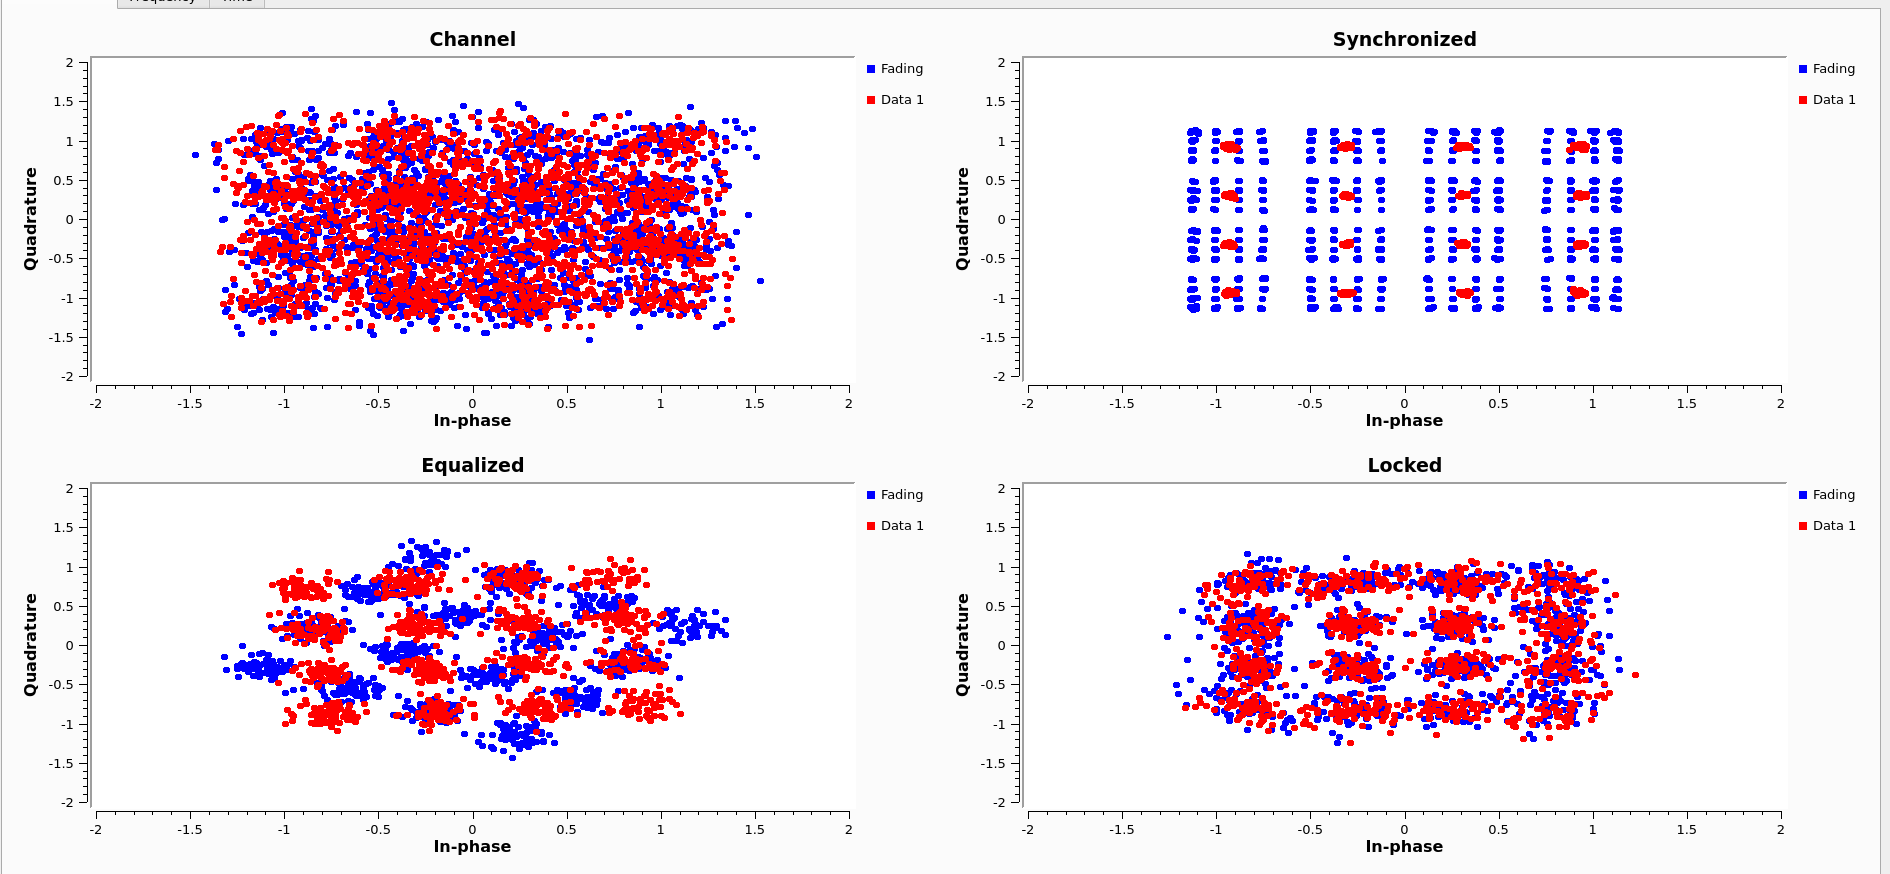
\includegraphics[width=10cm]{./figures/screenshots/QAM16_Fading_2.png}
 \end{figure}


\section{Hardware}

As Hardware we chosen the USRP B210 from Ettus Research, with the following specifications shown in Tab. \ref{tab:USRP B210 specifications}. Because this SDR is more than enough for our requires.

\subsection{Hardware setup}

The First Hardware set up was from the first SDR to the second, with a coaxial cable in between. 

The second was with the antennas. 2.4GHz. 

% To Do: Picture



\begin{table}[]
	%To DO sepzifikationen ampssen / genauer? https://www.ettus.com/wp-content/uploads/2019/01/b200-b210_spec_sheet.pdf
	%https://kb.ettus.com/B200/B210/B200mini/B205mini#FAQ
	\caption{USRP B210 specifications}
	\begin{tabular}[h]{|c|c|}
		\hline
		Dimensions & 9.7 x 15.5 x 1.5 cm \\
		\hline
		Ports &
2 TX , 2 RX, Half  or Full Duplex\\
		\hline
		RF frequencies & from 70MHz to 6GHz\\
		\hline
		Bandwidth & 200kHz-56MHz\\
		\hline 
		External reference input & 10 MHz \\
		\hline
	\end{tabular}
\label{tab:USRP B210 specifications}
\end{table}


\section{Measurements}



\section{Results}
